% !TeX root = ../main.tex
\cleardoublepage

%%% translation-related manual formatting
\newcommand{\apptitle}[1]{\parbox{0.9\linewidth}{\centering #1}\par\bigskip}
\newcommand{\appfigref}[2]{图~#1 -- #2~}
\newcommand{\appcite}[1]{\par\bigskip\apptitle{原文索引}\noindent\parbox{1\linewidth}{\small #1}}
\chapter{外文资料的书面翻译}

\apptitle{感性耦合等离子体环境下的静电卡盘特性瞬态分析}

\noindent 摘要:本文分析了感性耦合等离子体(ICP)环境下,用于在半导体工艺过程中夹持硅晶圆的J-R型静电卡盘(ESC)。我们提出了一个静电卡盘的双层等效电路模型,其组成为一较厚的整体层和一较薄的界面层。通过测量有/无晶圆时静电卡盘的伏安特性,可算出各层的等效电阻值,以及界面层两端等效电压。在静电卡盘上施加一斜坡电压信号,并测量其瞬态电流,积分即可得到界面层等效电容中储存的电荷量。另外,我们通过缓慢降低电压而使晶圆在氦气背吹作用下脱离卡盘的方式,在原位测量出了静电卡盘施加的静电力。用我们提出的等效电路模型预测的静电力与实际测量出的静电力相吻合。

\par\bigskip

\noindent \textbf{关键词:}J-R型;静电卡盘;感性耦合等离子体;双层模型

\par\bigskip

在有等离子体参与的半导体制程中,静电卡盘广泛用于真空环境中夹持硅晶圆。常用的静电卡盘分两种:库仑型[1-3],特点是使用绝缘体电介质层(体积电阻率$\rho > \SI{1e14}{\ohm\cm}$);以及Johnsen-Rahbek(J-R)型,特点是使用半导体电介质层($\rho = \SIrange{1e10}{1e12}{\ohm\cm}$)。静电吸附力由晶圆与静电卡盘中电极在高压作用下产生的异号电荷相吸引产生。与库仑型相比,J-R型静电卡盘可在较低电压下产生较强的吸引力,其原因主要是介电层表面微观不平度与晶圆接触后,缝隙间产生强电场。但J-R型静电卡盘吸附机理较复杂,且对界面层中的很多物理参数敏感,如电导率,表面微观不平度(亚显微级),甚至电极/晶圆的宏观平面度等;并且,使用J-R型静电卡盘的工艺存在一系列问题,如残余电荷带来的较差的可重复性,静态电流造成的晶圆表面镀膜破坏,以及将晶圆从静电卡盘表面卸下时,由顶针和残余电荷作用产生的晶片破损等。

为了能够消除这些缺点,我们需要增进对J-R型静电卡盘的理解,尤其是在等离子存在的实际工况下。在之前发表的文献[6]中,我们提出了射频偏压对低密度容性耦合等离子体(CCP)条件下的静电卡盘的伏安特性的影响。这里我们提出在高密度感性耦合等离子体(ICP)条件下的瞬态分析。接通电压时的瞬态电流的积分即为界面层电荷量,缓慢关断电压时,通过检测氦气背吹流量变化可测出静电吸附力。我们提出的双层等效电路模型可解释J-R型静电卡盘的特性。

实验使用一套ICP反应腔室[7],其圆柱形不锈钢制腔室中,使用\SI{13.56}{\MHz}射频放电激发\SI{0.1}{\torr}压强下的\ce{Ar}产生等离子体。在腔室内装有一\SI{200}{\mm}直径的J-R型静电卡盘。静电卡盘的电极材料为\ce{Mo},镶嵌在\SI{5}{\mm}厚的\ce{AlN}电介质层中,与接触表面距离\SI{0.54}{\mm}。接触表面总面积为电极投影面积的60\%(直接与晶圆接触的是静电卡盘表面上的凸台,高\SI{50}{\um},长宽\SI{2}{\mm},主要作用是为氦气冷却提供通道)。

\begin{figure}[tbhp]
\centering
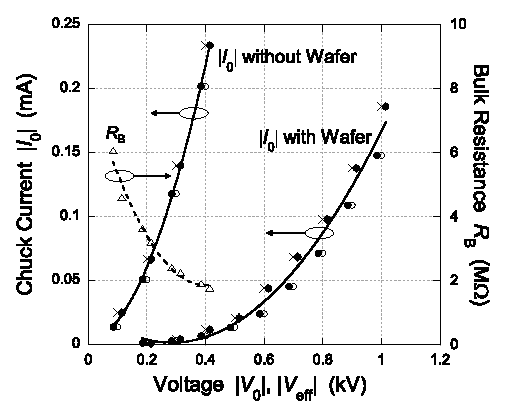
\includegraphics[width=0.7\linewidth]{_a/nagoya__1}
\caption*{图~A -- 1\hspace{1em}在有/无晶圆时,$I_0$与$\left|V_0\right|$的关系,以及无晶圆时$R_{\mathrm{B}}$的大小}
\end{figure}

首先,我们测量了\SI{600}{\W}放电,\SI{0.1}{\torr}压强产生的\ce{Ar}等离子体条件下,通过静电卡盘流向一直径\SI{200}{\mm}的硅晶圆的电流$I_0$与静电卡盘电压$V_0$(\SI{-1}{\kV}到\SI{+1}{\kV}之间)的函数关系。如\appfigref{A}{1}中``$\circ$''与``$\times$''所示,电压绝对值相同时,电流绝对值$\left|I_0\right|$在电压为负值时比电压为正值时要大。这个现象可用自偏压现象(self-bias effect)解释[6]:晶圆表面在ICP作用下,具有表面电势$V_{\mathrm{W}} \sim \SI{12}{\V}$,因此实际上静电卡盘中电极与晶圆之间的有效电压为$V_{\mathrm{eff}} = V_0 - V_{\mathrm{W}}$;即,$\left|V_0\right|$相等时,$-\left|V_0\right|$对应的有效电压更大。\appfigref{A}{1}中``$\cdot$''即为将电压修正为$V_{\mathrm{eff}}$的结果。$V_{\mathrm{eff}}/I_0$即为总电阻$R_{\mathrm{T}}$,由\ce{AlB}整体区电阻$R_{\mathrm{B}}$和接触电阻组成。%
当$\left|V_0\right|=\SI{0.4}{\kV}$时,$R_{\mathrm{T}} \sim \SI{40}{\Mohm}$;%
当$\left|V_0\right|=\SI{0.7}{\kV}$时,$R_{\mathrm{T}} \sim \SI{10}{\Mohm}$;%
当$\left|V_0\right|=\SI{1.0}{\kV}$时,$R_{\mathrm{T}} \sim \SI{6}{\Mohm}$;%
但这些数值明显大于通过体积电阻率估计出的整体层电阻$R_{\mathrm{B}} \sim \SI{3}{\Mohm}$(设$\rho=\SI{2e10}{\ohm\cm}$)。

通过测量观察到的在低电压下的高总电阻值说明在晶圆与静电卡盘中间存在较大的接触电阻。为了测出该接触电阻,首先要测量整体层电阻。将静电卡盘表面直接暴露在等离子体下,不加晶圆,测得其伏安特性如\appfigref{A}{1}。由于等离子体与静电卡盘接触较好,低电压下测得的电流较高。此时,整体层电阻即为$R_{\mathrm{B}}=\left|V_{\mathrm{eff}}\right| / \left|I_0\right|$,在\appfigref{A}{1}中用``$\Delta$''表示,可达\SI{2}{\Mohm}($V_0 > \SI{0.2}{\kV}$)。随着电压降低,仍可观测到电阻升高,这可能是由于静电卡盘与等离子体中仍存在的接触电阻升高造成的。

\begin{figure}[tbhp]
\centering
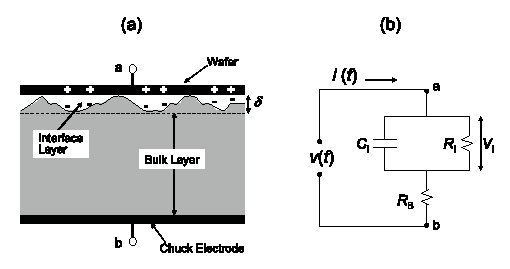
\includegraphics[width=0.7\linewidth]{_a/nagoya__2}
\caption*{图~A -- 2\hspace{1em}(a)\ J-R型静电卡盘双层模型\quad (b)\ 其等效电路}
\end{figure}

由\appfigref{A}{1}所示的测量数据,总结出\appfigref{A}{2}所示的J-R型静电卡盘双层模型,及其等效电路模型(\appfigref{A}{2(b)})。可将电极与晶圆之间的\ce{AlN}分为厚度$l=\SI{0.54}{\mm}$的整体层,其电阻为$R_{\mathrm{B}}$;以及厚度为$\delta$,较薄的界面层,其电阻为$R_{\mathrm{I}}$,电容为$C_{\mathrm{I}}=\varepsilon_0 S_{\mathrm{I}} / \delta$($S_{\mathrm{I}}$为待定的电容等效面积)。由于$\delta \ll l$,整体层的电容可忽略。总电阻$R_{\mathrm{T}}=R_{\mathrm{B}}+R_{\mathrm{I}}$。由伏安特性可知,$R_{\mathrm{I}}$随有效电压$V_{\mathrm{eff}}$非线性变化;这是J-R效应影响造成的,其机理可归结为在强电场下的电子场致发射现象[7,9,10]。整体层中流过的电流分布较均匀,但在通过界面层的若干个不规则接触点时,产生不均匀分布,并在接触点附近留下表面电荷$Q_0$;这样,晶圆与静电卡盘上的异号电荷形成了真空中的分布电容,其平均间隙为$\delta$;静电吸附力由此产生。随时间丢失的电荷由静态电流$I_0$补充,因此有如下稳态方程:
\begin{equation}\tag*{(A-1)}\label{eq:-a-1}
V_{\mathrm{I}}=R_{\mathrm{I}} I_0
Q_0=C_{\mathrm{I}} V_{\mathrm{I}}
\end{equation}

\begin{figure}[tbhp]
\centering
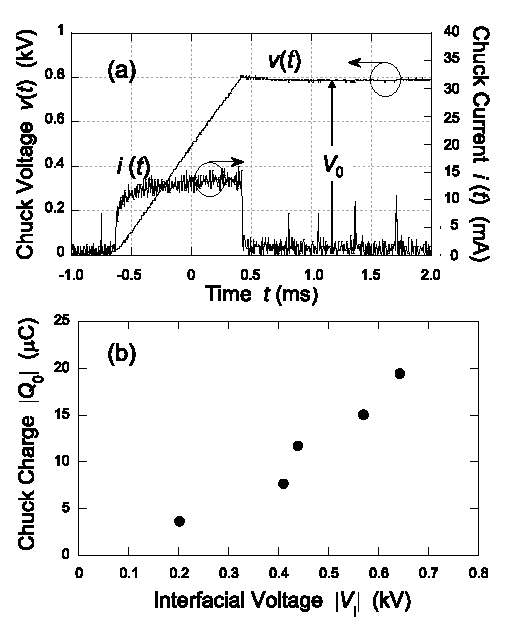
\includegraphics[width=0.5\linewidth]{_a/nagoya__3}
\caption*{图~A -- 3\hspace{1em}(a)\ $v(t)$与$i(t)$随时间变化\quad (b)\ 卡盘电荷$\left|Q_0\right|$随界面层电压$V_{\mathrm{I}}$变化关系 (\SI{600}{\W}、\SI{0.1}{\torr}条件下)}
\end{figure}

\begin{figure}[tbhp]
\centering
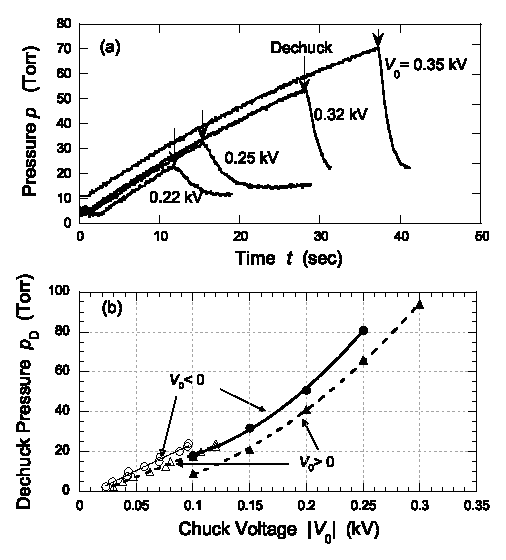
\includegraphics[width=0.5\linewidth]{_a/nagoya__4}
\caption*{图~A -- 4\hspace{1em}(a)\ 流量为\SI{10}{\sccm},电压不同时的氦气压强随时间变化关系\quad (b)\ 脱附压强随电压关系,负$V_0$为圆形点,正$V_0$为三角形点,恒流量法为实心点,恒压强法为空心点}
\end{figure}

为了得到稳态电荷$Q_0$,可在静电卡盘上施加一斜坡电压信号,并测量流过静电卡盘的瞬态电流,如\appfigref{A}{3(a)},电压$V_0$在$\tau_{\mathrm{R}} \sim \SI{1}{\ms}$内从0线性上升到\SI{0.8}{\kV}。电压关断时测得结果与接通时基本相同,只是电流方向相反(未在图中画出)。在图中,$\SI{-0.4}{\ms}<t<\SI{+0.4}{\ms}$时,可观测到较大(\SI{13}{\mA})的充电电流,之后迅速降到很小的稳态电流值(\SI{0.08}{\mA});偶尔出现的电流尖峰可能是由限流元件产生的。将测得的瞬态充电电流积分即可得到静电卡盘表面电荷量$Q_0$。如此可测得各电压$V_0$($<0$)下的表面电荷数据。定义界面层电压$V_{\mathrm{I}} = V_{\mathrm{eff}} - R_{\mathrm{B}} I_0$(即等效电路图中$C_{\mathrm{I}}$与$R_{\mathrm{I}}$两端的电压),其与$Q_0$关系如\appfigref{A}{3(b)}。可见,电荷量与电压并不成正比,其等效电容$C_{\mathrm{I}} = \left|Q_0\right| / \left|V_{\mathrm{I}}\right|$,在电容两端电压%
为\SI{0.2}{\kV}时为\SI{18}{\nano\farad},%
在\SI{0.64}{\kV}时为\SI{30}{\nano\farad}。%
这种电容随电压上升的现象,我们暂时认为是由于电压升高导致静电力升高,使得界面层厚度$\delta$缩小造成的。

通过原子力显微镜测量得到硅晶圆的表面粗糙度为\SIrange{0.8}{1.6}{\um}。考虑到介电层表面与晶圆表面的微观与宏观不平度,我们估计在电压为\SI{0.2}{\kV}时,界面层平均厚度$\delta \sim \SI{5}{\um}$;此时$C_{\mathrm{I}}=\SI{18}{\nano\farad}$,得到电容等效面积$S_{\mathrm{I}} \sim \SI{1.02e-2}{\m^2}$。另外,由于表面凸台影响,介电层与晶圆的实际接触面积为\SI{200}{\mm}直径圆形晶圆的60\%\footnotemark{},即$S_*=\SI{1.88e-2}{\m^2}$。

\footnotetext{译者注:此处原文意为“减小60\%接触面积”,有误,根据前后数据推断,实际应为“接触面积为整个晶圆的60\%”。}

为了检测静电吸引力,我们将一定压强的氦气通入晶圆与静电卡盘之间的空隙中。当作用在晶圆上的气体向上的压力稍微超过静电吸附力时,晶圆将脱离静电卡盘表面;此时氦气压力和/或流量将会发生改变。我们采用了两种测量方式:恒流量法和恒压强法。

如\appfigref{A}{4(a)},恒流量法是将氦气以固定的质量流量(\SI{10}{\sccm},即标况下\SI{10}{\cm^3\per\s})通入静电卡盘;共测试了4组电压下的情况:\SIlist[list-separator={,},list-final-separator={,以及}]{0.22;0.25;0.32;0.35}{\kV}。随着氦气流入,其压强逐渐升高;晶圆脱离后,由于气体大量漏出,压强突然降低。因此,图中标出的压强最高值,即晶圆即将脱离时的压强$p_{\mathrm{D}}$,就是气压与静电力平衡时的压强。\appfigref{A}{4(b)}中``$\bullet$''与``$\Delta$''分别表示$V_0 < 0$与$V_0 > 0$时,$p_{\mathrm{D}}$与$\left|V_0\right|$的关系。可见$V_0 < 0$时,吸附力更大。图中实线与虚线分别是两组数据的拟合曲线;其距离大约是\SI{25}{\V},与$V_{\mathrm{W}}$二倍大致相当,符合之前由\appfigref{A}{1}得出的结论。

在一系列试验过程中,我们发现前一次实验的结果会严重影响后一次,其原因为:当晶圆脱离后,在静电卡盘表面仍残留部分表面电荷,而这些电荷会影响后续试验。为了保证试验可重复性,我们在晶圆脱离后,将脱离的晶圆移至真空交换室(load-lock chamber),然后将静电卡盘暴露在\SI{0.1}{\torr}压强的\ce{Ar}等离子体中\SI{30}{\s},以去掉其表面残余电荷;这样即可保证采集数据可靠性。

\begin{figure}[tbhp]
\centering
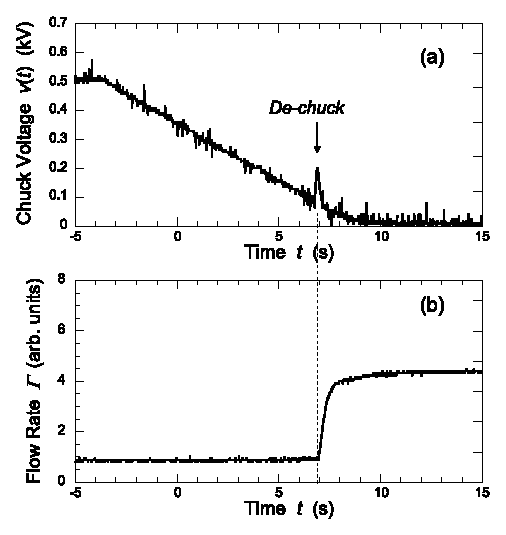
\includegraphics[width=0.7\linewidth]{_a/nagoya__5}
\caption*{图~A -- 5\hspace{1em}(a)\ $v(t)$随时间变化\quad (b)\ 氦气流量$\Gamma$随时间变化}
\end{figure}

在电压较低($\left|V_0\right| < \SI{0.15}{\kV}$)时,由于信号较小,而扰动较大,恒流量法测试精度下降。因此,在低电压区我们改用恒压强法来检测静电力。如\appfigref{A}{5},在维持氦气压力一定时,缓慢降低静电卡盘电压。氦气压强维持在$p = \SI{10}{\torr}$时,电压$V_0$在$t=\SI{-3.5}{\s}$时开始由\SI{0.5}{\kV}缓慢下降(约需10 s降至\SI{0}{\V})。\appfigref{A}{5(b)}中可见,在$t=\SI{7}{\s}$时,氦气流量突然增加,说明此时晶圆脱离,对应电压为\SI{0.07}{\kV}。脱离后,氦气流量迅速达到流量控制器允许的最大流量(\SI{50}{\sccm})。另外,在脱离时,可观测到电压值也出现一个尖峰,这是阻抗发生变化造成的。

当设置氦气恒定压强高于\SI{10}{\torr}时,晶片更早脱离,说明脱离时静电卡盘电压更大。反复试验即可得到气压与电压的函数关系,如\appfigref{A}{4(b)}中``$\circ$''和``$\Delta$''所示。当$\left|V_0\right|=\SI{0.1}{\kV}$时,更准确的恒定压强法获得的$p_{\mathrm{D}} \sim \SI{20}{\torr}$,约是恒流量法测试结果的两倍。

气体压强作用在晶圆上的面积$S_{\mathrm{M}}=\SI{1.26e-2}{\m^2}$(\SI{200}{\mm}直径晶圆的40\%)\textit{,除了电容等效面积$S_{\mathrm{I}}$}\footnotemark{}。因此,气压作用在晶圆上的合力为
\begin{equation}\tag*{(A-2)}\label{eq:-a-2}
F_{\mathrm{M}} = p_{\mathrm{D}} S_{\mathrm{M}}
\end{equation}
另一方面,使用测量得到的电容模型,可估计静电力为:
\begin{equation}\tag*{(A-3)}\label{eq:-a-3}
F_{\mathrm{E}} = \frac{D^2}{2 \varepsilon_0} S_{\mathrm{I}}
\end{equation}
其中电位移$D=Q_0/S_{\mathrm{I}}$。当静电卡盘电压$\left|V_0\right|=\SI{0.1}{\kV}$时,较准确的恒压强法测得$p_{\mathrm{D}} \sim \SI{20}{\torr}$,可得$F_{\mathrm{M}} \sim \SI{33.5}{\N}$;同条件下测得的表面电荷量$Q_0 \sim \SI{2.5}{\micro\coulomb}$,可得$F_{\mathrm{E}} \sim \SI{35.3}{\N}$。两者相差不大,在实验误差允许范围内,验证了晶圆脱离时$F_{\mathrm{M}}=F_{\mathrm{E}}$这一关系。

\footnotetext{译者注:原文此处语法不通,且由后面计算推断,此处并未从$S_{\mathrm{M}}$中扣除$S_{\mathrm{I}}$。}

总结:我们分析了ICP反应腔室中J-R型静电卡盘的基本特性,提出了由较厚阻性层与较薄容性层构成的双层电路模型,并通过加/不加晶圆的方法,用伏安特性法测量出了每一层的电阻值。加电压时的瞬态测量提供了一种新的测量静电卡盘表面电荷量的方式,并间接提供了估计静电力的方式(静电力与电荷量平方成正比)。我们还提出了一种利用氦气加压的较为精确地在原位测量静电力的方式;该法测量出的静电力与等效电路模型估测出的静电力相符较好。

\appcite{[1] SHIM G. I., SUGAI H. Temporal Analysis of Electrostatic Chuck Characteristics in Inductively Coupled Plasma[J]. Plasma and Fusion Research, 2008, 3: 028-028.} 


\clearpage


\apptitle{对夹持硅晶圆用的静电卡盘的基础研究}

\noindent 摘要:在半导体工业中,机械夹持晶圆的装置可能导致严重的问题。改用静电卡盘是可能解决这些问题的一种途径。我们研究了由交错电极和薄膜介电层组成的静电卡盘对硅片产生的静电吸引力的规律。当电压上升或介电层厚度降低时,静电力均上升。当交错电极的宽度和间距降低时,也能获得更强的静电力。实验表明当电极宽度和间距均为\SI{1}{\mm}、介电层为\SI{50}{\um}时,可获得最强的静电力:电压3.7 kV、吸引4英寸晶圆时,竖直方向静电力约为\SI{17}{\N}。在施加高压直流电压后,即使撤去电压,仍存在一些残余静电力,这种效应可用施加变频交流高压电的方式解决。

\par\bigskip

\noindent \textbf{关键词:}薄膜介电层;静电卡盘;静电力;硅晶圆夹持;交错电极

\par\bigskip

在半导体工业中,光学成像、化学气相沉积(CVD)、以及干法刻蚀等系统工作在真空条件下,而因为此时不能使用真空吸盘,机械夹持系统被广泛应用。但在搬运和夹持过程中,机械夹持系统对晶圆造成的污染可能会造成严重的问题。除此之外,机械夹持作用于晶圆的边缘处,因此可能无法保证其平整度。基于静电的夹持系统可能是一种解决这些问题的方法[1,2]。静电卡盘(ESC)可以在晶圆上施加分布夹紧力,足以使晶圆平整。另外,由于机械夹持系统在搬运时,为了避免颗粒污染,不能快速运动,而静电卡盘则无此问题,可以更快地搬运晶圆,提高产率。

虽然静电卡盘已经在坐标记录仪中应用了数十年[3],直到1970年代才由Wardly[4]提出可将其用于夹持硅晶圆。从此,因为上文所述的优点,大量半导体工业研究者开始投入到静电卡盘的研究中。这些研究的结果多数为专利;相比之下,学术刊物中出现的论文相对较少。

已经提出的静电卡盘种类很多[5],但基本上可分为两类:第一类静电卡盘需要将硅晶圆自身连接到高压电源上,称为“平行板电容器”(PPC,parallel-plate capacitor)型静电卡盘;第二类静电卡盘不需要硅晶圆与电源有电气连接,而是将电源连接到埋藏在介电层中的两个电极上,称为“交错电极”(IDE, interdigitated electrodes)型静电卡盘。在金属电极和硅晶片中间必须要有一层绝缘材料才能使其正常工作。

一般认为交错电极型静电卡盘产生的静电力要比平行板电容器型要弱,但交错电极型具有无需硅晶圆与电源有电气连接的优点,可大大简化整个系统。因此,我们选择交错电极型静电卡盘作为对象,通过改变其参数,以求获得尽可能强的静电力,来研究其基本特性。

\begin{figure}[tbhp]
\centering
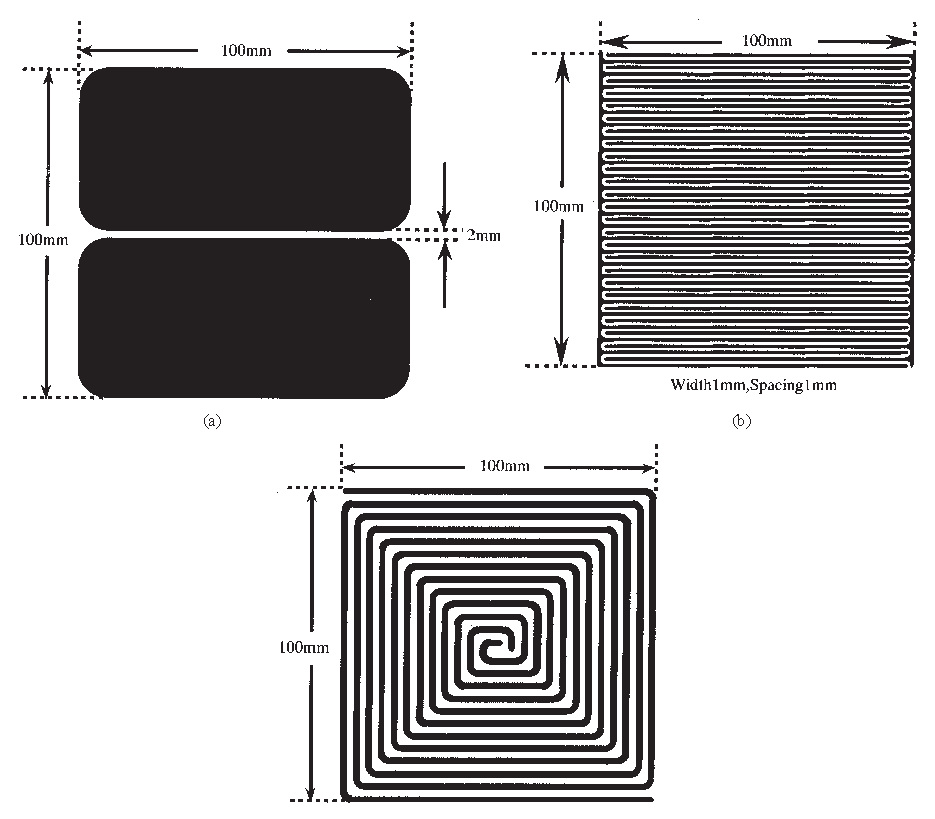
\includegraphics[width=0.7\linewidth]{_a/asano__1}
\caption*{图~A -- 6\hspace{1em}电极布置\quad (a)共平面型\quad (b)\ 平行交错\quad (c)\ 螺旋交错}
\end{figure}

\begin{figure}[tbhp]
\centering
\includegraphics[width=0.7\linewidth]{_a/asano__2}
\caption*{图~A -- 7\hspace{1em}测量系统}
\end{figure}

\begin{figure}[tbhp]
\centering
\includegraphics[width=0.7\linewidth]{_a/asano__3}
\caption*{图~A -- 8\hspace{1em}测力系统\quad (a)横向阻力\quad (b)\ 纵向吸引力}
\end{figure}

\begin{figure}[tbhp]
\centering
\includegraphics[width=0.7\linewidth]{_a/asano__4}
\caption*{图~A -- 9\hspace{1em}不同电极布置与牵引方向对力与电压关系的影响}
\end{figure}

\begin{figure}[tbhp]
\centering
\includegraphics[width=0.7\linewidth]{_a/asano__5}
\caption*{图~A -- 10\hspace{1em}随电极间距的变化关系:\quad (a)\ 力\quad (b)\ 电流}
\end{figure}

\begin{figure}[tbhp]
\centering
\includegraphics[width=0.7\linewidth]{_a/asano__5}
\caption*{图~A -- 10\hspace{1em}随电极间距的变化关系:\quad (a)\ 力\quad (b)\ 电流}
\end{figure}

\begin{figure}[tbhp]
\centering
\includegraphics[width=0.7\linewidth]{_a/asano__6}
\caption*{图~A -- 11\hspace{1em} 横向阻力随电压与绝缘薄膜厚度关系}
\end{figure}

我们测试了很多电极布置,其中部分如\appfigref{A}{6}:\appfigref{A}{6(a)}为共平面电极,下文简称A型;(b)与(c)为不同形状的交错电极,使用印刷电路板(PCB)工艺制成,下文分别简称B、C型。由于我们希望研究静电卡盘的基本特性,试验在大气条件下进行\footnotemark{}。在前期试验中,我们用一张透明幻灯片代替硅晶圆。当使用一张4英寸的硅晶圆做实验时,在晶圆与电极之间插入另一种塑料薄片,用于调节晶圆与电极之间的距离。

\footnotetext{译者注:逻辑不明但原文如此。}

测量系统如\appfigref{A}{7},可切换接通直流或交流电压,其中交流电压包括固定的\SI{50}{\Hz}以及由函数发生器经电压放大器产生的变频交流电压。静电吸引力由\appfigref{A}{8}所示系统测出。靠直接横向牵引晶圆或幻灯片可测出横向阻力,如\appfigref{A}{8(a)};在晶圆上方设置真空吸盘,用绳子通过滑轮,使用直线电机牵引,中间放置应变式力传感器,以此检测竖直方向静电吸引力。

为了探明电极方向性,我们首先横向牵引一张幻灯片。由于幻灯片的材料为PET(聚对苯二甲酸乙二酯),电极上并未覆盖额外的绝缘材料。试验中使用了不同形状参数的电极,如线宽和间距从\SI{0.5}{\mm}变化到\SI{3.0}{\mm}的B型电极。

\appfigref{A}{9}为横向阻力与电压关系,其中电极线宽与间距均为\SI{2}{\mm} mm。双共平面电极(A型)产生的阻力最小;当垂直于B型电极方向牵引时产生的阻力最大,当平行于电极方向时产生的阻力极其微弱;C型电极在各方向产生的阻力基本相等。B型电极显现出的方向性无法用简单的静电理论解释。由于B型电极产生的力高于其他两种,我们选择它作为进一步试验的对象。阻力与电极间距的关系如\appfigref{A}{10}.显然,间距越小,产生力越大;但当间距缩小至\SI{0.5}{\mm}时,试验结果并不理想,这可能是受到电极制造工艺的限制。因此,我们将间距与宽度均为\SI{1}{\mm}的B型电极选为试验基准。

由\appfigref{A}{10(b)}可看出,当电压增加至击穿时,电流迅速增加,为了防止击穿,增加静电吸引力,在电极上喷涂一层绝缘涂料(光刻胶GR-303);使用电容法测量其厚度为约\SI{8}{\um}。之后,又测量了阻力与喷涂的绝缘层厚度的关系,如\appfigref{A}{11};可看出绝缘层越薄,力越强。

\begin{figure}[tbhp]
\centering
\includegraphics[width=0.7\linewidth]{_a/asano__7}
\caption*{图~A -- 12\hspace{1em} 随PE薄膜厚度变化关系:\quad (a)\ 横向阻力\quad (b)\ 电流}
\end{figure}

\begin{figure}[tbhp]
\centering
\includegraphics[width=0.7\linewidth]{_a/asano__8}
\caption*{图~A -- 13\hspace{1em} 残余静电力}
\end{figure}

\begin{figure}[tbhp]
\centering
\includegraphics[width=0.7\linewidth]{_a/asano__9}
\caption*{图~A -- 14\hspace{1em} AC/DC电源对比:\quad (a)\ 力随电压变化\quad (b)\ 电流随电压变化}
\end{figure}

\begin{figure}[tbhp]
\centering
\includegraphics[width=0.7\linewidth]{_a/asano__10}
\caption*{图~A -- 15\hspace{1em} 残余静电力与电流随频率变化关系}
\end{figure}


虽然我们将多种不同材料的绝缘层放置在电极和晶圆中间测试,其中只有PE(聚乙烯)薄膜有多种厚度,因此,大量实验中使用了不同厚度的PE薄膜。由于电极是用PCB工艺刻蚀而成,在电极间存在\SI{35}{\um}高的凸台,导致在施加高压时击穿产生的气隙。因此我们使用硅胶填充这一空隙。横向阻力随电压关系如\appfigref{A}{12}。可见,当PE绝缘层厚度为\SI{50}{\um}高时,可以产生相当强的阻力;当使用更薄的绝缘层时,其表面稳定性变差,经常随晶圆一起被拖动,导致阻力降低。

在使用直流电压试验时,发现残余电荷对试验有很大影响:切断电源较长时间后仍存留有横向阻力。\appfigref{A}{13}是一次测量的结果:初始阻力为\SI{9}{\N}(电压3 kV,绝缘层厚度\SI{50}{\um}),而切断电源12小时后,仍有\SI{4}{\N}阻力残留。为了解决此问题,我们尝试使用高压交流电源。当使用\SI{50}{\Hz}交流电源时,能够消除残余阻力\footnotemark{},但因为电容反复充放电,产生较大反应电流。因此,我们使用函数发生器和电流放大器产生低频高压交流电压。\appfigref{A}{14}比较了使用直流、\SI{1}{\Hz}、\SI{10}{\Hz}电源时产生的阻力和电流大小。如\appfigref{A}{15}所示,采用低频交流供电时,残余阻力大大减小。

\footnotetext{译者注:原文中此处逻辑混乱,疑似为日文直译造成。}

\begin{figure}[tbhp]
\centering
\includegraphics[width=1\linewidth]{_a/asano__11}
\caption*{图~A -- 16\hspace{1em}  静电吸引力随直流电压变化关系:%
\quad (a)\ 介电层厚\SI{16}{\um}%
\quad (b)\ 介电层厚\SI{23}{\um}%
\quad (c)\ 介电层厚\SI{50}{\um}%
}
\end{figure}

为了测量竖直方向上的静电吸引力,使用真空吸盘来夹持晶圆;试验中需确保真空吸盘与晶圆对中。尽管采取了这样的措施,测得的吸引力散布相当大,因此对多组数据取平均值分析。如\appfigref{A}{16},测量了不同电压、不同绝缘层厚度下的吸引力大小,并在图中表示出了平均值。发现静电吸引力较强\footnotemark{}。残余吸引力仍存在,同样可用变频交流供电法消除。

\footnotetext{译者注:原文如此。}

从初期试验中可看出,交错电极型静电卡盘能在塑料薄膜上产生较大的横向阻力,且该阻力随电极间隙减小而增强。然而由于漏电流和击穿强度等因素影响,可能存在一个最优的间隙大小,在我们的试验中得出该大小为\SI{1}{\mm};该值可能与电极制造工艺有关。
当使用\SI{1}{\mm}间隙的电极时,可以在晶圆上产生大于\SI{15}{\N}的静电吸引力。通过改变绝缘层材料与厚度,可以进一步增强静电吸引力。
当电极间存在绝缘材料(包括硅胶)时,即使切断电源,仍存在残余电荷,进而产生残余静电力;可用施加变频交流电压的方式减小这一影响。

\appcite{[1] ASANO K., HATAKEYAMA F., YATSUZUKA K. Fundamental study of an electrostatic chuck for silicon wafer handling[J]. Industry Applications, IEEE Transactions on, 2002, 38(3): 840-845.}